%!TEX root = ../Final_Assignment_SP_ML4IM_2023.tex
\chapter{Methods}
\label{ch:methods}

% ausführlich, am wichtigsten
% NOT FINAL - unsure about section structure and names
% hendrik und maxi


The scope of this project is to create a model which is abale to detect insects in a video stream. To achive this goal, a combination of computer vision methods was used to preprocess the video stream. The following sections will describe the all methods used in this project.

The generell workflow for this project was to first collect (and label) and then to preprocess the data using computer vision methods. After that the data was converted to a typ usable for YOLO and finally a model was trained on the preprocessed data. The preprocessing and training was a iterative process to find the best possible model.

\section{Data Collection}

The collection of the raw video stream, containing the DVS and RGB streams, was done by team CVMLS of Prof. Dr. Benjamin Risse from the Institute of Geoinformatics at the University of Münster.

The provided datasets were then labeled by all students of the study project "Machine learning meets insect monitoring" in the winter semester 2023/2024. The labeling was done using labelbox, a platform for labeling images and videos. 

At the end of the data collection phase there were 34 videos, containing both streams stack on top of each other (later individual videos for each stream), with corresponding labels. The labels were in the form of bounding boxes around the insects in the video.

\section{Data Preprocessing}

The proprocessing of the video streams was done using computer vision methods provided by the OpenCV library. Our group was tasked with the preprocessing of the RGB stream.\\
Note that all of the following methods were not used in the sequence they are presented here and also are not all used in the same preprocessing. These are the basic methods used for different preprocessings or in combination with each other, but never all at the same time.\\
To see all used combinations see Chapter~\ref{chap:results}.

\textbf{Substraction} \\
The substraction is the simple method of substracting one image from another. The idea behind this was to subtract the background of the images and only keep the moving parts.\\
The results were a black and white image that showed the difference between the two images.\\

\begin{figure}[htbp]
    \centering
    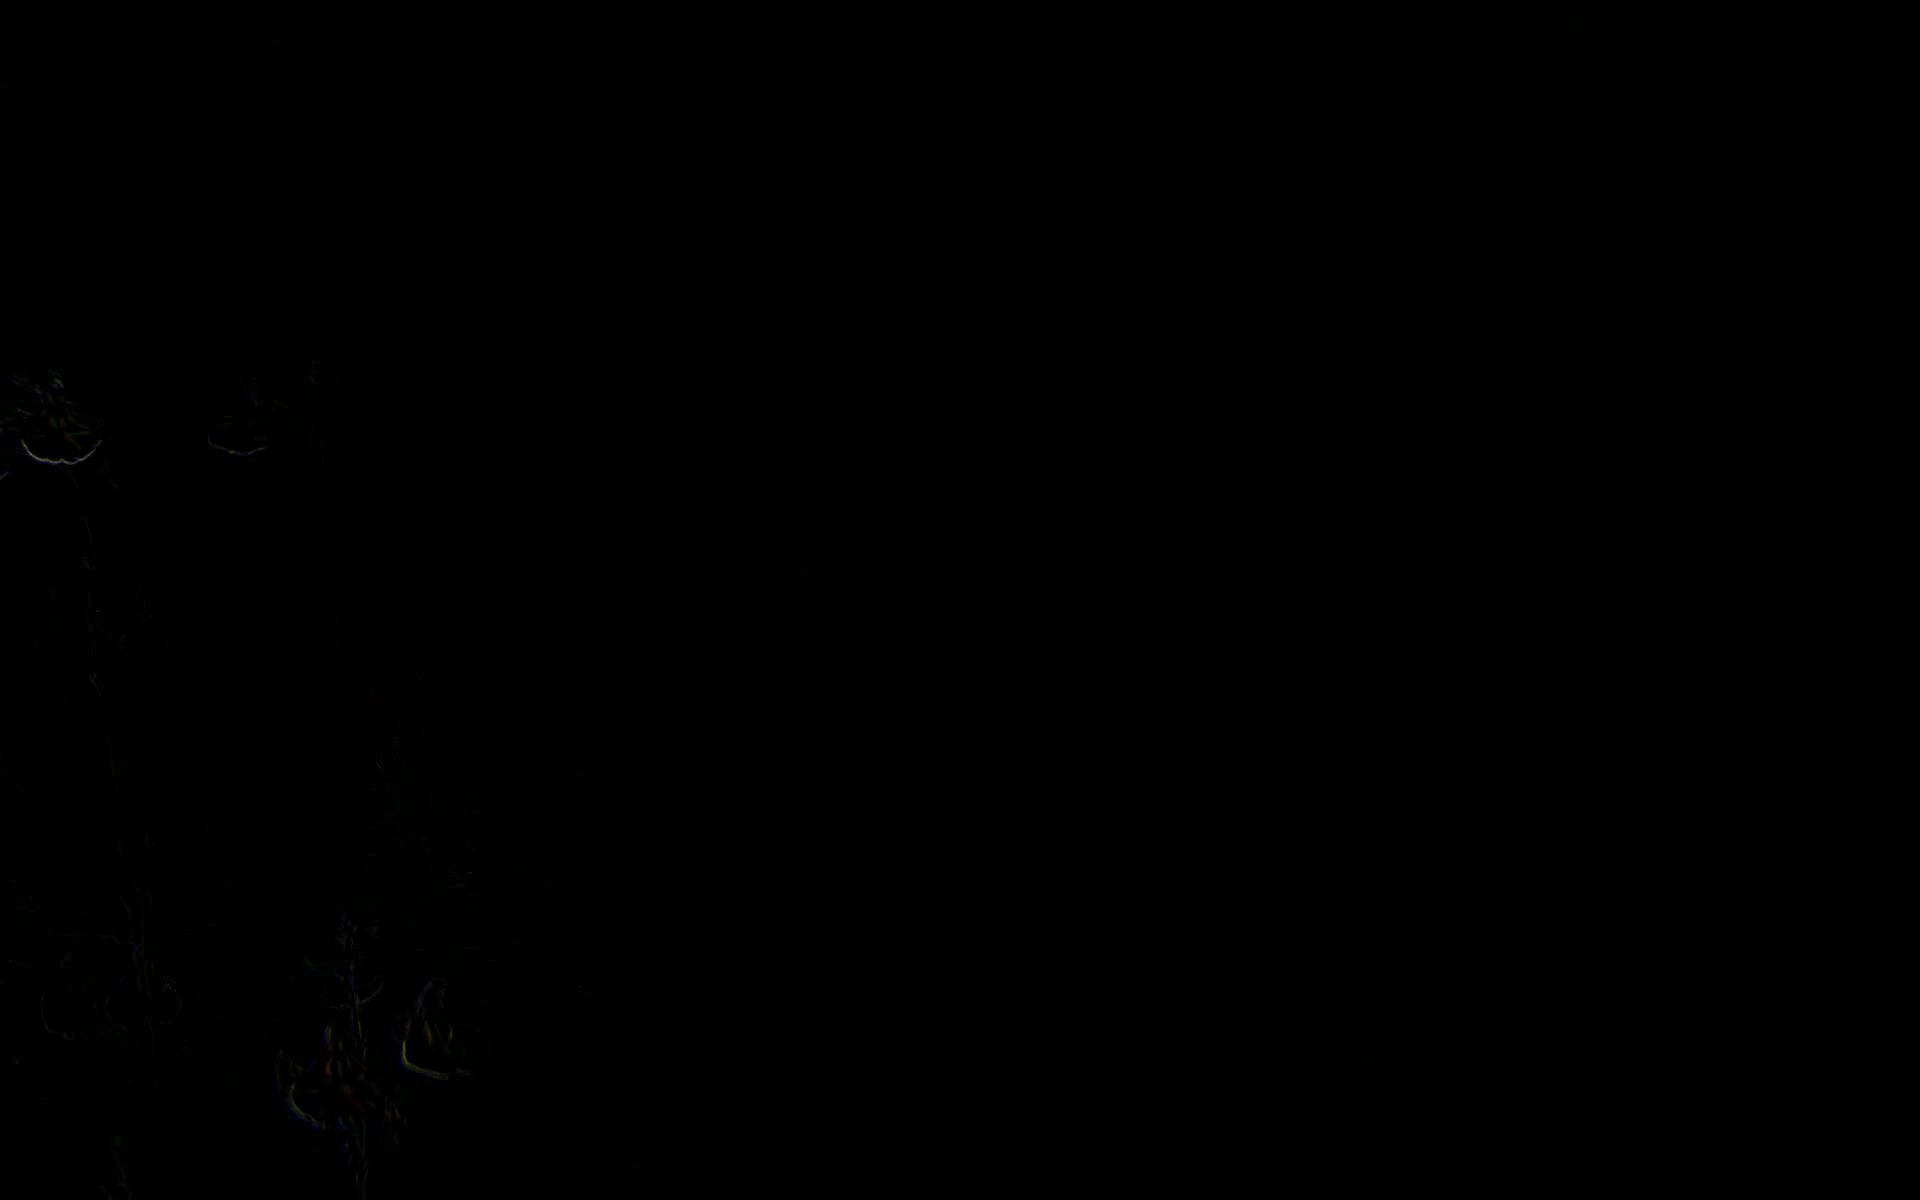
\includegraphics[width=0.5\textwidth]{../images/img_002_002309_Sub.png}
    \caption{The output of the subtraction preprocessing}
\end{figure}

\textbf{Background Subtraction} \\
The background subtraction method is a more advanced version of the substraction method. The idea was again to remove the background from the image. Here you dont substract the two consecutive images but rather have a background model that is subtracted from the image.\\
This Method is somewhat comparable with the dvs stream, as it also only shows the moving parts of the image.\\

\begin{figure}[htbp]
    \centering
    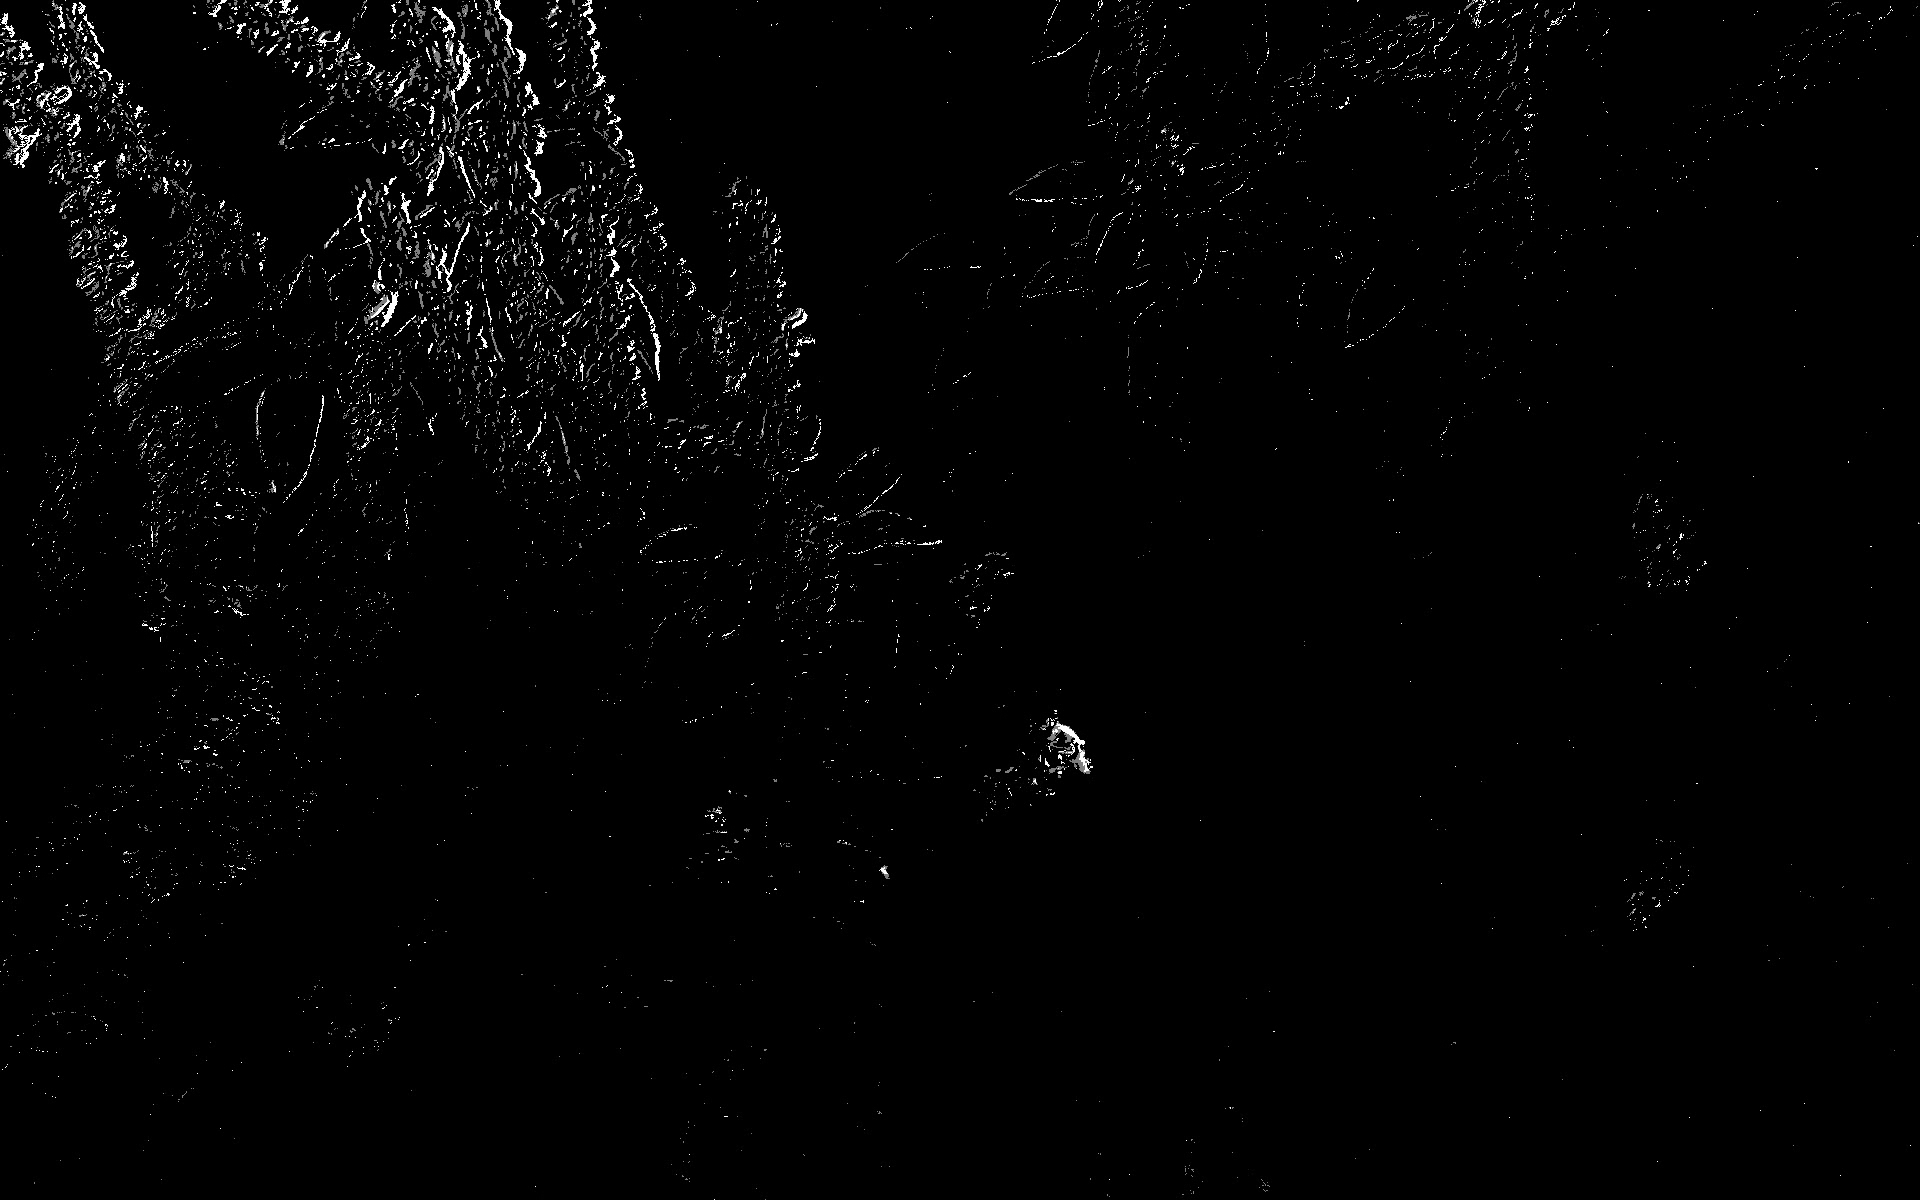
\includegraphics[width=0.5\textwidth]{../images/img_002_002309_BackSub.png}
    \caption{The output of the background subtraction preprocessing}
\end{figure}


\textbf{RGB to HSV} \\
The RGB to HSV method converts the RGB image to a HSV image. The HSV color space is a cylindrical color space containing three components: hue, saturation, and value. The idea behind this method was to have another color space to work with.\\
This also allows to change each component individually, for example enhance the saturation.\\

\begin{figure}[htbp]
    \centering
    \includegraphics[width=0.5\textwidth]{../images/img_002_002309_HSV.png}
    \caption{The output of the RGB to HSV preprocessing}
\end{figure}

\textbf{Time offset} \\
Time offset is a method to create each frame from three images (each gets its own channel) which have a time offeset. This offest can range from just one frame to multiple frames. The idea behind this method was to capture the movement of the insects. The more frames are between the iamges the bigger is the captured movement. This also creates a change to capture insects that are sitting still for a certain amount of time.\\

\begin{figure}[htbp]
    \centering
    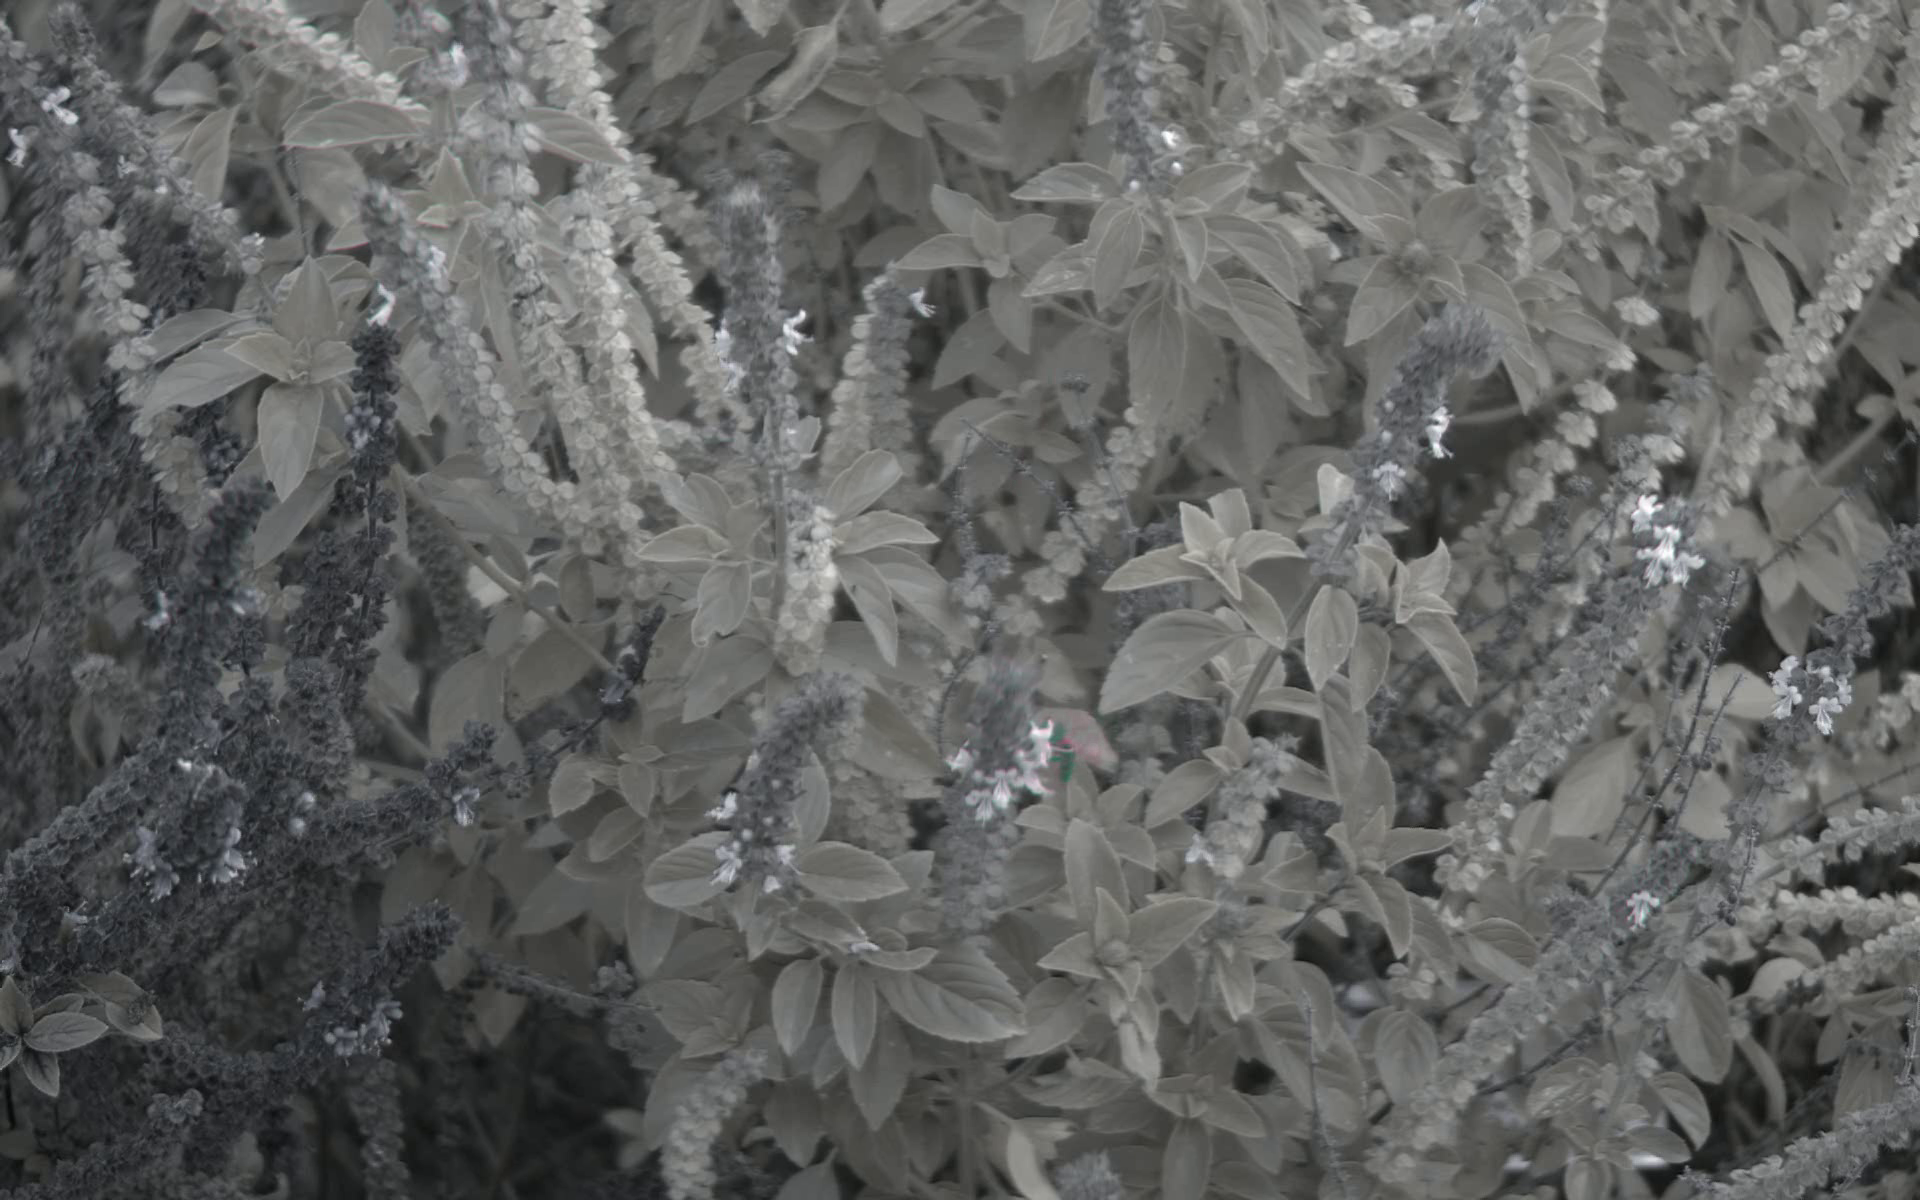
\includegraphics[width=0.5\textwidth]{../images/img_002_002309_OffsetBy10.png}
    \caption{The output of the time offset (by 10) preprocessing}
\end{figure}

\section{Data Processing}

After pre-processing the videos, the data was converted into a format that could be used to train a model. The videos are available as mp4 files and the labelbox data is available as an ndjson file. This ndjson contains information about the bounding box and its associated frame. The YOLO training algorithm requires the images and the bounding boxes to be in a specific format, which is performed by the build dataset script. The basic script to perform this data processing was written by Jakob Marten Danel, a fellow student in the Study Project, and has been adapted to the rgb data and also includes a bounding box conversion. \\

\textbf{Dataset building}

The build dataset script iterates through every video in the input folder and extracts the frames from the video. The script then checks if the frame is in the labelbox data and if so, it creates a txt file with the bounding box information. The script then moves the frame to the corresponding folder in the output folder. The aim is to have the videos as individual frames and the corresponding bounding boxes per frame in a txt file of the same name. In addition, the videos are randomly divided into training and validation data in a ratio of 80:20. A yaml file describes the folder structure and the locations where yolo finds the images and txt files. \\

\textbf{Converting Bounding boxes}

The process of adapting insect labels from DVS streams to RGB data involved several steps to ensure accurate alignment. First, bounding boxes were applied to the DVS data only. Due to differences in image capture between the event-based camera and the RGB camera, as well as differences in resolution (1920x1200 for RGB versus 1280x720 for DVS), a conversion process was required.

Several iterations of conversion were tried before the result was satisfying. The first attempt involved a simple translation of the bounding boxes by one unit in the x and y axes. Subsequent analysis revealed that the DVS stream captured an enlarged section of the scene. To address this discrepancy, a second version of the conversion was developed that scaled the box coordinates relative to their proximity to the centre of the image.

Despite improvements, problems persisted, particularly at the edge of the image, where distortion was more distinct. As a result, a new approach was adopted using a homographic transformation to adjust for image distortion. This transformation produced a homography matrix that provided insight into the distortion between the RGB and DVS images.

Ultimately, the final conversion method used the homography matrix to adjust the data, with additional scaling along the x and y axes to ensure alignment. This approach effectively aligned the insect labels between the DVS and RGB streams.

\section{Model Training}

% Hier könnte auch die erklörung für die Bounding Boxen hin
% Hier müsste eine kurze Erklärung zum Training stehen
